\documentclass[11pt]{amsart}
\usepackage{amsmath,amssymb,booktabs,graphicx,hyperref,longtable}
\title[Values of the Erd\H{o}s--Selfridge function through 400]{Further values of the Erd\H{o}s--Selfridge function\\and a GPU algorithm for computing them}
\author{Alexander Eastwood}
\address{Independent researcher}
\date{September 14, 2026}
\begin{document}
\begin{abstract}
We report $g(378),\ldots,g(400)$ for the Erd\H{o}s--Selfridge function, extending the
Sorenson--Sorenson--Webster frontier of 377. A complete table through 400 and paired
search records accompany this note. The computation uses partial-prime-power CRT
wheels, strip-mined CUDA enumeration and residue filters. Fresh exact checks verify
admissibility of all 400 values; checks of 108 completed block records support the
recorded exhaustive searches for the 23 frontier terms. These record checks are
distinguished from an independent exhaustive replay of minimality.
\end{abstract}
\maketitle
\section{Definition and prior work}
Define $g(k)=\min\{n>k+1:p(\binom nk)>k\}$, where $p(m)$ is the least prime factor
of $m$. Earlier tables and algorithms appear in \cite{EES74,SW92,LSW97,SSW20,SSW21}.
The 2021 addendum gives values through 377. Our complete data file preserves the
389 entries in the OEIS b-file retrieved on September 14, 2026, and adds 390--400.
Repository publication and OEIS editorial approval are separate events.
\section{Wheel and GPU enumeration}
By Kummer's theorem, $p\nmid\binom nk$ precisely when every base-$p$ digit of $k$
is at most the corresponding digit of $n$. Write $t_p=\lfloor\log_p k\rfloor+1$
and $k=\sum_{i<t_p}a_{ip}p^i$. The condition is periodic modulo $p^{t_p}$, with
$\prod_{i<t_p}(p-a_{ip})$ admissible residues. Following \cite{SSW20}, choose partial
prime powers $p^{T_p}$, $0\le T_p\le t_p$, by a knapsack strategy. They give
\[
N=\prod_p p^{T_p},\qquad R_N=\prod_p\prod_{i<T_p}(p-a_{ip}).
\]
CRT enumerates those $R_N$ wheel-admissible residues. A prime with $T_p<t_p$ remains
in the residual filters. GPU threads reconstruct mixed-radix residues with exact
128-bit integer arithmetic, then strip-mine one ring so successive candidates
reuse the outer CRT work. Early residue filters reject most candidates; surviving
candidates are checked by the frozen arbitrary-precision Python reference.

Blocks $[tN,(t+1)N)$ are scanned in increasing $t$, and the minimum valid survivor
in the first nonempty block is returned. The final confirmations for 397 and 399
used word-mask filters retaining original candidate identities and compatible
checkpoint coverage. The second run for each term uses a different wheel and
modulus; these runs nevertheless share software components.
\section{Verification scope}
The release validator freshly checks all 400 witnesses with the frozen Kummer
reference and with exact binomial coefficients: 17,391 prime-divisor tests.
For 378--400 it checks 108 unique completed block records across 46 runs,
including wheel-derived moduli and residue counts, consecutive blocks, survivor
intervals and hashes, and the absence of earlier valid survivors in the lists.
Repeated identical checkpoint rows are counted once. Reconstructed historical
audit rows retain their provenance labels. The 397 confirmation includes reused
completed coverage; it is not additional novel search work.

Witness checks establish admissibility, not minimality. Minimality relies on the
correctness and completeness of the exhaustive enumeration and filtering.
Two different wheels provide a cross-check, not a formal proof of implementation
correctness. Survivor hashes authenticate the lists but do not certify that no
candidate was omitted. No fresh exhaustive CPU or GPU replay was performed as
part of this publication audit. Complete independent reproduction requires
re-enumerating the recorded wheels.
\section{Results}
\begin{longtable}{r r c}
\toprule $k$ & $g(k)$ & Blocks: primary / confirm \\
\midrule
378 & 11243132307156301763663607287294 & 9 / 6 \\
379 & 161870983573549868804425756301179 & 1 / 1 \\
380 & 10462825184429793014317942235516 & 1 / 1 \\
381 & 12870452058086999925869938534781 & 1 / 1 \\
382 & 33595253716498387794413412981758 & 14 / 4 \\
383 & 540148968489634107903617360993663 & 2 / 1 \\
384 & 347602760349418009297709548536219 & 1 / 2 \\
385 & 327295190388354179623724094491095 & 1 / 1 \\
386 & 13244365243698813468350652166046 & 1 / 1 \\
387 & 17088927744279024569389598842319 & 1 / 1 \\
388 & 1379978640683593021393172825519 & 1 / 1 \\
389 & 4171959526360182919803787001674199 & 2 / 1 \\
390 & 1967924476778959819324408694516718 & 1 / 1 \\
391 & 1407678907549820296859900034849791 & 2 / 3 \\
392 & 2149910863290282683111595748554173 & 4 / 1 \\
393 & 8221905832123087594889003885519 & 1 / 1 \\
394 & 26940132483154282770968897574794 & 1 / 1 \\
395 & 70422314661266035686410669061023 & 2 / 1 \\
396 & 7350984493848874781629926017999 & 1 / 2 \\
397 & 7282852096749166908452220090055597 & 5 / 5 \\
398 & 358644756463853013270803607289823 & 2 / 1 \\
399 & 1463367633345557449307696345739199 & 7 / 5 \\
400 & 58305842808280308870124770403739 & 2 / 3 \\
\bottomrule
\end{longtable}
\begin{figure}[ht]
\centering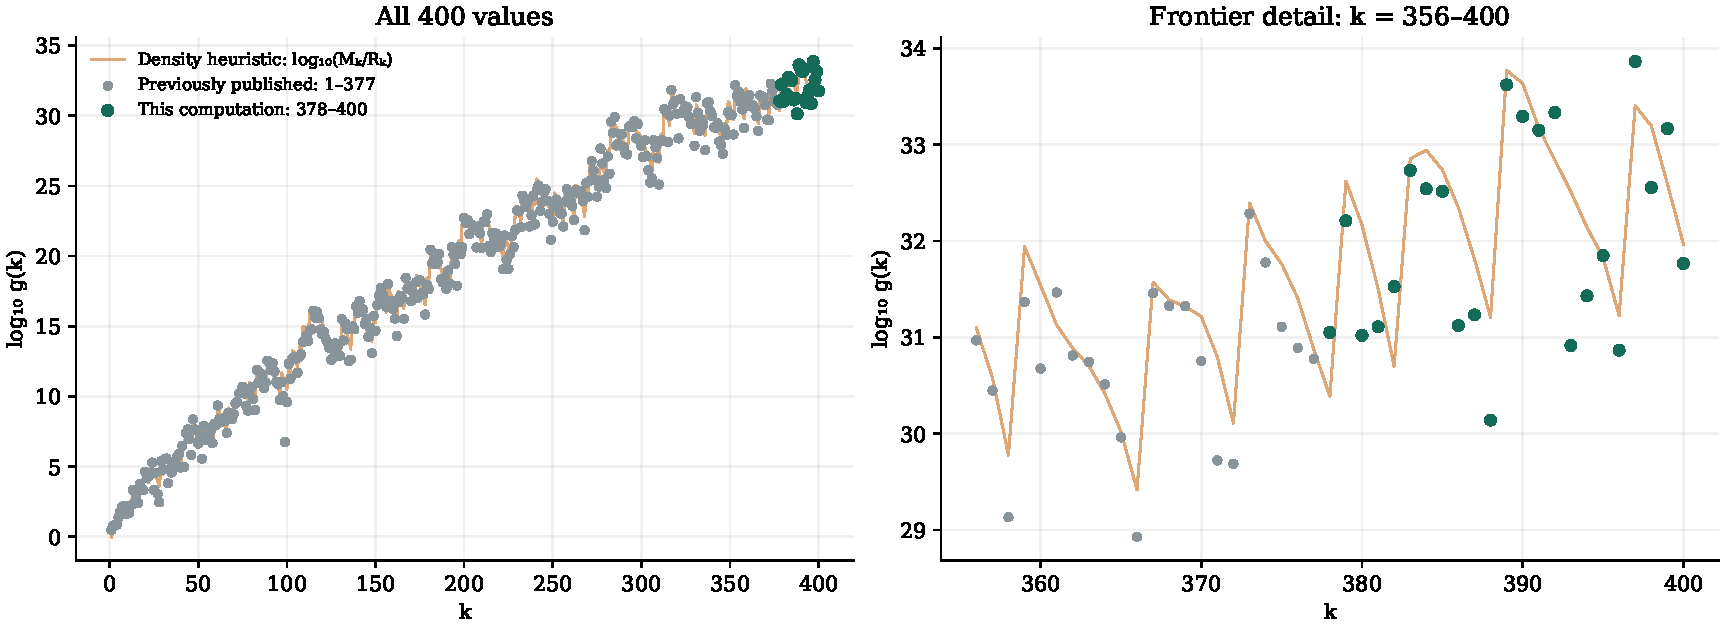
\includegraphics[width=\linewidth]{terms_growth.pdf}
\caption{All 400 values and detail for 356--400. Gray: 1--377; green: 378--400.
The orange curve is $\log_{10}(M_k/R_k)$, where
$M_k=\prod_{p\le k}p^{t_p}$ and $R_k=\prod_{p\le k}\prod_{i<t_p}(p-a_{ip})$.
This density heuristic is not a bound or a minimality certificate.}
\end{figure}
\section{Reproduction}
The complete table, paired records, source hashes and CPU validator are at
\url{https://github.com/AlexanderEastwood/erdos-selfridge}.
Run \texttt{python3 harness/verify\_release.py} for the release checks, and
\texttt{python3 harness/replay\_release.py 399 confirmation} to print a fresh
exhaustive GPU replay command. Adding \texttt{--execute} starts that scan; large
terms may take days. The replay uses archived v9 for the recorded mathematical
scope rather than reproducing historical timings. The last word-mask records
also bind their source files by per-run SHA-256 manifests; older summaries do
not have equally complete runtime manifests.

No cross-hardware timing comparison or new distributional conclusion is claimed
in this release. The earlier Zenodo archive predates this update. Computational
development and drafting used AI assistance under the author's direction. This
repository note does not assert arXiv publication or OEIS editorial acceptance.
\section*{Acknowledgments}
The author thanks Hoi Tran, Roscoe Pershall, and David Whitfield of Parkrose High School, Portland,
Oregon, and his father, Charles Eastwood, whose teaching fostered a lasting interest in
mathematics. He also thanks B. Sorenson, J.~P. Sorenson and J. Webster, whose algorithm this
work builds on directly.

\begin{thebibliography}{9}
\bibitem{EES74} E.~F. Ecklund Jr., P. Erd\H{o}s, J.~L. Selfridge, A new function associated with the prime factors of $\binom nk$, Math.\ Comp.\ 28 (1974) 647--649.
\bibitem{SW92} R. Scheidler, H.~C. Williams, A method for tabulating the number-theoretic function $g(k)$, Math.\ Comp.\ 59 (1992) 251--257.
\bibitem{LSW97} R.~F. Lukes, R. Scheidler, H.~C. Williams, Further tabulation of the Erd\H{o}s--Selfridge function, Math.\ Comp.\ 66 (1997) 1709--1717.
\bibitem{SSW20} B. Sorenson, J.~P. Sorenson, J. Webster, An algorithm and estimates for the Erd\H{o}s--Selfridge function, ANTS XIV, Open Book Series 4 (2020) 371--385.
\bibitem{SSW21} B. Sorenson, J.~P. Sorenson, J. Webster, An algorithm and estimates for the Erd\H{o}s--Selfridge function: addendum, arXiv:1907.08559v3 (2021).
\bibitem{OEIS} OEIS Foundation, Sequence A003458, \url{https://oeis.org/A003458}.
\end{thebibliography}
\end{document}
